\forRevThree{In this section we present the model, as well as background on sketches. 
%and the Maximum Merging (MM) method~\cite{yang2018elastic} for compressing the CM sketch. 
Finally, we detail related work.
}

\forRevThree{
\subsection{Model}
}

\forRevThree{
We consider the incoming packets in the network as originating from a single \emph{stream}. A \emph{flow} is defined to be a sub-stream with common packet headers, e.g., grouping together all packets containing the same 5-tuple. A \emph{measurement} is some function $f$ computed over the stream, e.g., returning the distinct number of flows in the stream. As streams are generally too large to maintain in memory~\cite{cormode2011sketch}, accuracy is traded off for a lower memory footprint~\cite{CountMin, agarwal2013mergeable, KMV} by algorithms called \emph{sketches}. Several sketches have the \emph{mergeability} property that refers to the ability for computing a sketch over a stream by merging sketches over substreams.}

\forRevThree{
As mentioned previously, measurements are conducted in switches all over the network. We model this by splitting the stream into disjoint sub-streams observed by \emph{ingestion nodes}, where parts of the same flow may be observed by different ingestion nodes. Once the nodes have a sketch ready to be sent (e.g.,  periodically or upon receive a specific signal) they propagate their local sketch or a summary for it to a \emph{central node}~\cite{huang2017sketchvisor, li2016flowradar, liu2016one}, which merges all sketches to provide the desired measurement.}

\subsection{Background}

In this section, we present the Count-Min sketch, the KMV sketch, and the HLL sketch. We present the Maximum Merging (MM) method.

\subsubsection{The Count-Min Sketch (CM)} \label{sktc-ssec:backgroound-CM}

Estimating flow size is a required capability 
in many networking applications,
in fields as diverse as accounting, monitoring, load balancing and filtering, and even beyond networking. Counting the exact size of every flow is often challenging due to a typically large number of active flows at a specific time, making it difficult to maintain a counter-per-flow within a memory accessible at the line rate.
There can be two types of errors in the estimation of a flow size: Overestimations and underestimations. The state-of-the-art data structure for flow size estimation is the Count-Min (CM) sketch  suggested by Cormode and Muthukrishnan in 2005~\cite{CountMin}.

\forRevThree{The CM sketch is instantiated with parameters $\epsilon$ and $\delta$, where the flow size estimation is within error $\epsilon$ with probability at least $1-\delta$. It is comprised of a two dimensional} array of counters of size $d \times w$, where $d = \lceil \ln{1 / \delta}\rceil$ and $w=\lceil e / \epsilon \rceil$, and all counters are initialized to 0. Note that the number of columns is determined by the error (and, conversely, the error is determined by the number of columns), and the probability is determined by the number of rows.
A set of $d$ hash functions are used to map a flow to $d$ counters, one in each of its rows. 
Upon a flow arrival, each of these counters is incremented.

To estimate the size of a flow, its $d$ selected counters are considered and the size is estimated as the minimum among these counters. Since multiple flows can contribute to the same counter, the computed value is \ingreen{potentially} larger than the exact one. \ingreen{In case other flows contributed to all $d$ counters then an overestimation is derived}. 
CM completely avoids underestimations. A tradeoff exists between the level of accuracy and the allocated memory such that more memory reduces collisions among flows. Similarly, reducing the number of flows improves accuracy.

\inblue{An important property of the CM sketch is the \emph{mergeability} property: Two CM sketches with parameters $(\epsilon,\delta)$ can be merged by element-wise addition to a sketch with the same parameters.} \forRevThree{We capitalize on this property which enables computing a sketch over the whole stream by merging sketches over substreams, which has also been exploited in previous work~\cite{stylianopoulos2020delegation, rinberg2019fast, cormode2011algorithms}.}

 %However, to the best of our knowledge there are no known results on how to completely avoid flow size overestimations even when the number of flows is small.


\begin{figure}[!t]%[!ht]
	\centering
		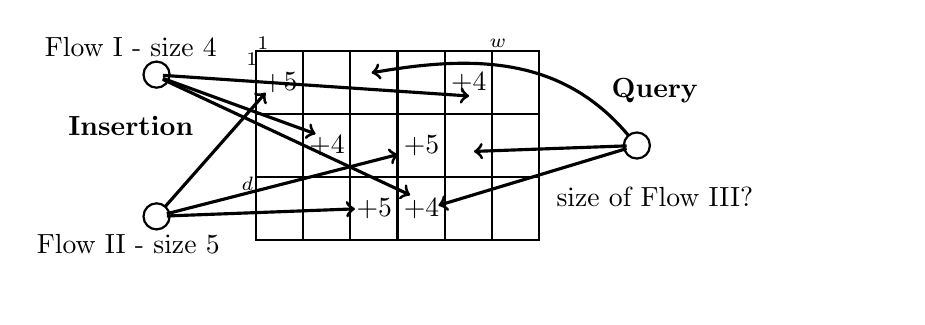
\begin{tikzpicture}
 \foreach \c/\i [count=\n] in  
        {white/4,white/0, white/0,white/0,white/9,white/0} 
           \node[draw,fill=\c,minimum height=0.8cm,minimum width = 0.6cm,xshift=(\n+2.1)*0.6cm](B\n){};
            \foreach \c/\i [count=\n] in  
        {white/4,white/0, white/0,white/0,white/9,white/0} 
           \node[draw,fill=\c,minimum height=0.8cm,minimum width = 0.6cm,xshift=(\n+2.1)*0.6cm, yshift =0.8cm](B\n){} ;
            \foreach \c/\i [count=\n] in 
        {white/4,white/0, white/0,white/0,white/9,white/0} 
           \node[draw,fill=\c,minimum height=0.8cm,minimum width = 0.6cm,xshift=(\n+2.1)*0.6cm, yshift =1.6cm](B\n){} ;
         \foreach \j [count=\m] in  
        {0,1,2,3,4,5,6,7,8,9,10,11,12,13,14} 
           \node[] (q\m) at (\m*0.5cm,0.36) {}; 
\node[text width=0.75cm, anchor=west, right] at (0.73,-1.0) {};
\node[text width=0.75cm, anchor=west, right] at (2.31,-1.0) {};
 \foreach \j [count=\m] in  
        {1,1,2,3,4,5,6,7,8,9,10,11,12} 
           \node[] (z\m) at (\m*0.5cm,-0.46) {}; 
\node[text width=3.5cm, anchor=west, right] at (-1.25,2.05) {Flow I - size 4};
\node[draw,circle,scale=1.0, thick] at (0.30,1.7) {}; 
\node [] (n0) at (0.25,1.7) {};
\node [] (z1) at (4.40,1.42) {};
\node [] (z2) at (2.45,0.9) {};
\node [] (z3) at (3.65,0.11) {};
\draw[line width=0.04cm, ->] (n0) -- (z1);
\draw[line width=0.04cm, ->] (n0) -- (z2);
\draw[line width=0.04cm, ->] (n0) -- (z3);

\node[text width=0.5cm, anchor=west, right] at (2.11,0.8) {$+4$};
\node[text width=0.5cm, anchor=west, right] at (3.91,1.6) {$+4$};
\node[text width=0.5cm, anchor=west, right] at (3.31,0.0) {$+4$};
\node[text width=0.5cm, anchor=west, right] at (2.71,0.0) {$+5$};
\node[text width=0.5cm, anchor=west, right] at (3.31,0.8) {$+5$};
\node[text width=0.5cm, anchor=west, right] at (1.51,1.6) {$+5$};
%\draw[->] (n0) -- (-0.4,+0.46);
%\draw[->] (n0) -- (q3);

\node[text width=0.5cm, anchor=west, right] at (1.45,2.10) {\scriptsize $1$};
\node[text width=0.5cm, anchor=west, right] at (4.40,2.10) {\scriptsize $w$};

\node[text width=0.5cm, anchor=west, right] at (1.31,1.90) {\scriptsize $1$};
\node[text width=0.5cm, anchor=west, right] at (1.25,0.32) {\scriptsize $d$};


\node[draw,circle,scale=1.0, thick] at (0.30,-0.1) {};
\node[text width=3.5cm, anchor=west, right] at (-1.35,-0.45) {Flow II - size 5};
\node [] (nl) at (0.30,-0.1) {};
\node [] (nl1) at (1.80,1.6) {};
\node [] (nl2) at (3.5,0.72) {};
\node [] (nl3) at (2.95,0.0) {};
\draw[line width=0.04cm, ->] (nl) -- (nl1);
\draw[ line width=0.04cm, ->] (nl) -- (nl2);
\draw[line width=0.04cm, ->] (nl) -- (nl3);


\node[draw,circle,scale=1.0, thick] at (6.40,0.8) {};
\node[text width=3.5cm, anchor=west, right] at (5.25,0.15) {size of Flow III?};
\node [] (n2) at (6.4,0.8) {};

\node [] (n21) at (2.90,1.7) {};
\node [] (n22) at (4.2,0.72) {}; 
\node [] (n23) at (3.75,0.0) {};
%\draw[blue, line width=0.04cm, ->] (n2) --  (n21);
\draw [->, line width=0.04cm] (n2) to [out=130,in=10] (n21);
\draw[line width=0.04cm, ->] (n2) -- (n22);
%\draw [->, line width=0.04cm] (n2) to [out=200,in=290] (n23);
\draw[line width=0.04cm, ->] (n2) -- (n23);
\node[text width=3.5cm, anchor=west, right] at (-0.95,1.05) {\textbf{Insertion}};
\node[text width=3.5cm, anchor=west, right] at (5.95,1.5) {\textbf{Query}};
%\draw[->] (nl) -- (q3);
%\draw[->] (nl) -- (q8);
%\node[text width=3.5cm, anchor=west, right] at (4.60,1.75) {Flow III - size 1};
%\node[draw,circle,scale=1.0, thick] at (5.29,1.4) {};
%\node [] (n2) at (5.3,1.3) {};
%\draw[->] (n2) -- (q8); 
%\draw[->] (n2) -- (q11); 
%\node[draw,circle,scale=1.0, thick] at (2.59,-1.4) {};
%\node[text width=4.0cm, anchor=west, right] at (1.51,-1.7) {size of Flow II?};
%\node [] (n3) at (2.6,-1.3) {};
%\draw[->] (n3) -- (z3);
%\draw[->] (n3) -- (z8);
\end{tikzpicture}
\caption{\label{sktc-fig:CM} The Count-Min sketch (CM)~\cite{CountMin}, allowing flow size estimation. \inred{Each flow is mapped to a single counter in each row. Flow I is mapped to counter 5 in row 1, counter 2 in row 2, and counter 4 in row 3. The mappings are presented in the figure.} A flow size is estimated as the minimum among the counters it is mapped to by a set of hash functions.}	
\end{figure}

The CM  is illustrated in Figure~\ref{sktc-fig:CM}. Flows I, II  of size 4, and 5, respectively, are recorded in the sketch (shown on the left side). Each flow increases the value of $d=3$ counters by its size.  The size of Flow III (right side) is estimated by querying the CM  as the minimal among the $d$ counters it is mapped to.

%As for every sketch, the estimation generated from the Count-Min sketch is imperfect and can be overestimated.
\inred{While, as mentioned, the CM can observe overestimations~\cite{CountMin}}, the accuracy guarantees can be described as follows:
When using CM with width $w$ and depth $d$ the estimation $\hat{f}$ of flow $f$ satisfies with probability $1-\delta$
\[\hat{f} \leq f + \epsilon N.\]
Here, $N$ is the number of packets in the measured stream, $\epsilon$ holds $w = \left\lceil \frac{e}{\epsilon} \right\rceil$ (for Euler's number $e$) and $\delta$ holds $d= \left\lceil \ln\frac{1}{\delta} \right\rceil$.

\subsubsection{KMV (\emph{K-minimum-values}) Sketch}  \label{sktc-ssec:kmv}

Another essential capability in network monitoring is the ability to estimate the number of distinct flows, called stream cardinality. Counting the exact stream cardinality is generally challenging in high traffic rate, making it hard to save some unique data for each flow and quickly identify whether a flow has previously appeared or not. 

The $K$-minimum-values sketch (KMV)~\cite{giroire2009order, KMV} uses a hash function $h$ that maps every flow uniformly to $[0,1]$. For a parameter $k$, the sketch maintains the minimal $k$ observed values for flows so far. Let $h_1,...,h_k$ be those $k$ minimal calculated values such that $h_1<h_2<...<h_k$. The \emph{KMV} sketch provides its cardinality estimation as $\frac{k}{h_k}$. This estimation is based on the fact that the $k$ order statistics of group uniformly randomized in the range $[0,1]$ is equal to $\frac{k}{n+1}$. The error of the algorithm is $\frac{1}{\sqrt{k}}$, i.e.  for $m$ flows, the KMV sketch estimation $m'$ satisfies $\left|\frac{m-m'}{m}\right| = O(\frac{1}{\sqrt{k}})$.

\begin{figure}[!t]%[!ht]
	\centering
	

\tikzset{every picture/.style={line width=0.75pt}} %set default line width to 0.75pt        

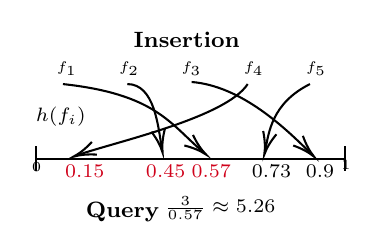
\begin{tikzpicture}[x=0.75pt,y=0.75pt,yscale=-1,xscale=1]
%uncomment if require: \path (0,300); %set diagram left start at 0, and has height of 300

%Straight Lines [id:da2080794547555267] 
\draw    (101.5,100.67) -- (250.5,100.67) ;
%Straight Lines [id:da6803929792177787] 
\draw    (101.5,94.67) -- (101.5,106.67) ;
%Straight Lines [id:da0782789730692306] 
\draw    (250.5,94.67) -- (250.5,106.67) ;
%Curve Lines [id:da9195899812176473] 
\draw    (114.5,64.67) .. controls (159.12,69.52) and (166.1,83.78) .. (182,97.4) ;
\draw [shift={(183.5,98.67)}, rotate = 219.47] [color={rgb, 255:red, 0; green, 0; blue, 0 }  ][line width=0.75]    (10.93,-3.29) .. controls (6.95,-1.4) and (3.31,-0.3) .. (0,0) .. controls (3.31,0.3) and (6.95,1.4) .. (10.93,3.29)   ;
%Curve Lines [id:da2342594252069674] 
\draw    (145.5,64.67) .. controls (158.66,64.67) and (160.33,84.99) .. (162.15,95.73) ;
\draw [shift={(162.5,97.67)}, rotate = 258.69] [color={rgb, 255:red, 0; green, 0; blue, 0 }  ][line width=0.75]    (10.93,-3.29) .. controls (6.95,-1.4) and (3.31,-0.3) .. (0,0) .. controls (3.31,0.3) and (6.95,1.4) .. (10.93,3.29)   ;
%Curve Lines [id:da7520327389763415] 
\draw    (176.5,63.67) .. controls (200.63,65.6) and (221.96,86.15) .. (234.2,98.37) ;
\draw [shift={(235.5,99.67)}, rotate = 225] [color={rgb, 255:red, 0; green, 0; blue, 0 }  ][line width=0.75]    (10.93,-3.29) .. controls (6.95,-1.4) and (3.31,-0.3) .. (0,0) .. controls (3.31,0.3) and (6.95,1.4) .. (10.93,3.29)   ;
%Curve Lines [id:da8707723296036518] 
\draw    (203.5,64.67) .. controls (192.89,81.07) and (138.5,92.82) .. (121.23,99.01) ;
\draw [shift={(119.5,99.67)}, rotate = 338.2] [color={rgb, 255:red, 0; green, 0; blue, 0 }  ][line width=0.75]    (10.93,-3.29) .. controls (6.95,-1.4) and (3.31,-0.3) .. (0,0) .. controls (3.31,0.3) and (6.95,1.4) .. (10.93,3.29)   ;
%Curve Lines [id:da46923256267070834] 
\draw    (233.5,64.67) .. controls (215,73.92) and (213.61,88.3) .. (211.93,96.74) ;
\draw [shift={(211.5,98.67)}, rotate = 284.04] [color={rgb, 255:red, 0; green, 0; blue, 0 }  ][line width=0.75]    (10.93,-3.29) .. controls (6.95,-1.4) and (3.31,-0.3) .. (0,0) .. controls (3.31,0.3) and (6.95,1.4) .. (10.93,3.29)   ;

% Text Node
\draw (98,101) node [anchor=north west][inner sep=0.75pt]   [align=left] {{\tiny 0}};
% Text Node
\draw (247,100) node [anchor=north west][inner sep=0.75pt]   [align=left] {{\tiny 1}};
% Text Node
\draw (110,52.4) node [anchor=north west][inner sep=0.75pt]  [font=\tiny]  {${\displaystyle f_{1}}$};
% Text Node
\draw (140,52.4) node [anchor=north west][inner sep=0.75pt]  [font=\tiny]  {${\displaystyle f_{2}}$};
% Text Node
\draw (170,52.4) node [anchor=north west][inner sep=0.75pt]  [font=\tiny]  {${\displaystyle f_{3}}$};
% Text Node
\draw (200,52.4) node [anchor=north west][inner sep=0.75pt]  [font=\tiny]  {${\displaystyle f_{4}}$};
% Text Node
\draw (230,52.4) node [anchor=north west][inner sep=0.75pt]  [font=\tiny]  {${\displaystyle f_{5}}$};
% Text Node
\draw (147,38) node [anchor=north west][inner sep=0.75pt]   [align=left] {\textbf{{\footnotesize Insertion}}};
% Text Node
\draw (230,102) node [anchor=north west][inner sep=0.75pt]   [align=left] {{\scriptsize 0.9}};
% Text Node
\draw (204,102) node [anchor=north west][inner sep=0.75pt]   [align=left] {{\scriptsize 0.73}};
% Text Node
\draw (175,102) node [anchor=north west][inner sep=0.75pt]  [color={rgb, 255:red, 208; green, 2; blue, 27 }  ,opacity=1 ] [align=left] {{\scriptsize 0.57}};
% Text Node
\draw (114,102) node [anchor=north west][inner sep=0.75pt]  [color={rgb, 255:red, 208; green, 2; blue, 27 }  ,opacity=1 ] [align=left] {{\scriptsize 0.15}};
% Text Node
\draw (153,102) node [anchor=north west][inner sep=0.75pt]  [color={rgb, 255:red, 208; green, 2; blue, 27 }  ,opacity=1 ] [align=left] {{\scriptsize 0.45}};
% Text Node
\draw (100,74.4) node [anchor=north west][inner sep=0.75pt]  [font=\scriptsize]  {$h( f_{i})$};
% Text Node
\draw (124,120) node [anchor=north west][inner sep=0.75pt]   [align=left] {\textbf{{\footnotesize Query}}};
% Text Node
\draw (162,117.4) node [anchor=north west][inner sep=0.75pt]  [font=\scriptsize]  {$\frac{3}{0.57} \approx 5.26$};


\end{tikzpicture}

    \caption{The $K$-minimum-values sketch (KMV) \cite{giroire2009order, KMV}, allowing cardinality estimation. The cardinality is estimated by dividing $k$ with the $k$'th minimal hashed value, (here $k=3$ with recorded values shown in red).}
    \label{sktc-fig:kmv-example}
\end{figure}

The KMV is illustrated in Figure \ref{sktc-fig:kmv-example}. There are five flows recorded in the sketch, each maps to a different value in the range of $[0,1]$. Here $k=3$ so that only the three minimal values are stored. When flows' cardinality is queried, the sketch finds the largest value that is currently stored, which is $0.57$ and returns $\frac{k}{0.57} = \frac{3}{0.57} \approx 5.26$ distinct flows.

\subsubsection{HyperLogLog for Cardinality Estimation}
\label{sktc-ssec:HyperLogLog}

% \begin{algorithm}[!h]
% \DontPrintSemicolon
% \KwIn{
% Stream of elements $A = (a_1, \ldots, a_k)$.
% }
% \KwOut{
% Estimated number of distinct elements in $A$
% }
% $M[0] = \ldots = M[m-1] = 0$, $d= \log_2(m)$, $\alpha_m  = 0.7213 / (1+1.079/m)$ for $m \ge 128$;

% \For{$a_i \in A$} {
% $(b_1, \ldots, b_d, b_{d+1}, \ldots, b_{d+t}) = h(a_i)$ \\
% $j =  (b_1, \ldots, b_d)$\\
% $M[j] = \max(M[j], \rho((b_{d+1}, \ldots, b_{d+t})))$
% }
% $Z = \Big(\sum_{j = 0}^{m-1} {2^{-M[j]}}\Big)^{-1}$\\
% \Return $\alpha_m  \cdot m^2 \cdot Z$\\
% \caption{The \emph{HyperLogLog} algorithm for cardinality estimation~\cite{Flajolet07hyperloglog}}
% %for estimating number of distinct elements
% \label{sktc-Alg_HyperLogLog}
% \end{algorithm}



HyperLogLog (HLL)~\cite{Flajolet07hyperloglog,heule2013hyperloglog} is another popular algorithm for cardinality estimation.
As a building block, it relies on the Flajolet–Martin method of estimating the number of distinct elements~\cite{flajolet1983probabilistic, LogLog}. They propose computing a hash value $h(a_i)$ for each element $a_i$ and a value $\rho(h(a_i))$ that indicates the index of the first non-zero bit upon considering the binary representation of $h(a_i)$, starting from the least significant bit. 
The HLL holds an array $M$ of $m=2^d$ counters. For an element $a_i$, a counter is selected based on the $d$ left-most bits in $h(a_i)$ and this counter is potentially updated based on the next $t$ bits in  $h(a_i)$. 
The use of hashing ensures that repeated elements in the stream imply the same values and thus cannot increase the counter values. Finally, \inblue{the cardinality estimation} computed based on the $m$ counters is:
\[\alpha_m  \cdot m^2 \cdot \big(\sum_{j = 0}^{m-1} {2^{-M[j]}}\big)^{-1}.\]
$\alpha_m$ is approximated as:
\[\alpha_m=\begin{cases}
0.673 & m=16 \\
0.697 & m=32 \\
0.706 & m=64 \\
\frac{0.723}{1+\frac{1.079}{m}} & m \geq 128
\end{cases}\]
as shown in~\cite{Flajolet07hyperloglog}.
% The pseudocode for the HLL algorithm is shown in Algorithm ~\ref{sktc-Alg_HyperLogLog}. 

\subsubsection{Maximum Merging (MM)} \label{sktc-ssec:mm}

\inblue{
Previous work by Yang et al. has presented the Maximum Merging (\textbf{MM})~\cite{yang2018elastic} method, a method for compressing CM before transmission over the network. In this method, the CM sketch is compressed from size $w$ to $w'$, where $w'$ is a divisor of $w$. Column $i$ is added to column $(i \mod w')$. If $w = r \cdot w'$, the CM sketch is compressed by} \ingreen{a factor}  \inblue{$r$ earlier to its transmission over the network.
}

\forRevThree{
While this method maintains the lookup speed of the original CM sketch, a limitation of this method is the requirement that $w'$ be a divisor of $w$.
%}
%\forRevThree{ 
Even more important, in the common  scenario of multiple measurements,  
the MM scheme compresses all sketches equally regardless of the amount of traffic each of them observes. 
We indicate that this scheme can lead to under utilized bandwidth. For example, if the two node processed different portions of the stream, an identical compression implies over-compression of the sketch that observes more traffic, leading to a higher overall error.} %We explain that typically the sketch that observed a smaller portion of the traffic can be further compressed without affecting much the overall error. }

%Furthermore, if the traffic distribution was not equal, i.e., one node processed a much larger portion of the stream, the MM scheme applies equal compression to both nodes. For example, consider the case where node 1 processes $90\%$ of the stream and node 2 processes $10\%$ of it. Under MM compression, both nodes send a similar summary size.

%We propose having node 2 highly compress its summary, and node 1 compressing it less than in MM. While in this case node 1 sends a larger summary than in MM, the sum of the compressed sizes in MM is greater than the sum of our proposed compressed sizes, while the error remains similar. I.e., we use less bandwidth while achieving a similar error.

\subsection{Related Work} \label{sktc-ssec:related-work}

Common sketch solutions focus on the trade-off of speed, accuracy, and memory (e.g.,~\cite{CountMin, cormode2011sketch, metwally2005efficient, sivaraman2017heavy, estan2003new,  9667240, 9068483, Rottenstreich21} and more). However, they generally consider only a single node ingesting the entire stream.
The introduction of software-defined networks (SDN) allows for deploying
centralized algorithms for maintaining and collecting information about network
operations~\cite{yu2013software}. These solutions typically have a centralized controlled merging
of incoming data from ingestion nodes. Network-wide measurements have
been widely studied~\cite{afek2018detecting,anderson2017high,li2016flowradar,harrison2020carpe}. These solutions, however, do not consider the size of control packets sent to the controller -- they do not take into account that these control packets may worsen existing congestion~\cite{zhang2010optimizing, benson2010understanding}.

 Shrivastava et al.\cite{shrivastava2016time} presented time adaptive sketches and discussed the need for having recent data more accessible. In \cite{harrison2018network}, Harrison et al. presented a network-wide scheme of detecting heavy-hitters while considering the reporting communication overhead. \cite{harrison2020carpe} presented a method of heavy-hitters detection that used probabilistic summary reporting to decrease control packets during DDoS attacks. These two works emphasize that minimizing summaries size is critical and can have a major influence on network performance. By using methods of our paper, network operators can create larger sketches and excess the need for time-reliant sketches. 


Recently,~\cite{FPFZCM} suggested methods for accurate flow size estimation in the Count-Min sketch (CM)  without overestimation, that apply when the number of flows of non-zero size is bounded. 
Yang et al. presented the Maximum Merging (\textbf{MM})~\cite{yang2018elastic}, a method for compressing CM before transmission over the network. MM allows providing estimations under a range of traffic characteristics implying various bandwidth constraints. The main limitation of this method is that it can only compress the CM to a constant $w'$ which divides the width $w$.
\forRevThree{
MM does not deal with two aspects that we find important for making it practical. It refers to a single sketch and does not discuss the compression of multiple sketch instances and in particular how to compute various compression ratios for such sketches based on the traffic. Likewise, it is focused solely on the CM. In this work, we study the common scenario of multiple distributed sketches and refer in addition to CM also to other common sketches. 
}


\forRevThree{
Our methods utilize similar patterns to the original sketches, therefore our proposed sketches and techniques may have the potential to be implemented on programmable switches. 
For example, the following sketches have been implemented using the Tofino architecture~\cite{tofino}:
the CM sketch~\cite{namkung2021telemetry}, the Quantiles sketch~\cite{ivkin2019qpipe}, and more~\cite{zhang2021cocosketch, hang2019interleaved, zeno2020swishmem}.}

%\forRevThree{As mentioned, the Elastic Sketch~\cite{yang2018elastic} presented a compression method for sketches, to adapt to available network bandwidth using the MM technique, detailed in Section~\ref{sktc-ssec:mm}. MM allows providing estimations under a range of traffic characteristics implying various bandwidth constraints. It refers to a single instance of the CM Elastic Sketch However, unlike our SKTC compression approach,  and does not discuss how to use multiple instances of the Elastic Sketch for a single distributed sketch. We refer to the MM technique as a baseline scheme in the evaluations.}


%UnivMon~\cite{liu2016one} and NitroSketch~\cite{NitroSketch} summarize streams in a sketch that can later answer multiple measurement tasks. The SKTC compression approach can be generalized to such sketches, while the analysis of the ideal resize factors can be generalized to refer jointly to the accuracy of multiple tasks. \inblue{To the best of our knowledge, only the Elastic Sketch adapts to \inred{available network bandwidth}~\cite{yang2018elastic} using the MM technique. It is proposed to continuously provide estimations under all traffic characteristics, \inred{i.e., provide estimations under all network scenarios, e.g., in low-bandwidth conditions when the network is undergoing a DDoS attack. They do not discuss how to use multiple instances of the Elastic Sketch for a single distributed sketch. Our main point of comparison with the Elastic Sketch is the MM compression technique.}}